\subsubsection{Aufbau und Entwicklung des Frontends}  
\label{sec:Aufbau und Entwicklung des Frontends-1}

Durch eine zusätzliche Javascript-Bibliothek „Vue-resource“ werden asynchrone Anfragen an die Backend-API geschickt, die die passenden Daten liefert. Um dem Nutzer ein wenig Arbeit abzunehmen werden sobald ein editierbares Feld verlassen wird die Daten auch in der Datenbank direkt aktualisiert. Vorausgesetzt es handelt sich um valide Daten.
Für jede Komponente wird das entsprechende Template anhand der ID definiert.
Die Daten werden anhand des data-Attributs festgelegt und können dann mithilfe von „this“ aufgerufen werden. 
Des Weiteren können auch Methoden definiert werden, welche aufgerufen werden können. Um eine Komponente mit Daten zu initialisieren wird die „created“-Eigenschaft verwendet. Diese wird sobald die Komponente erstellt wurde aufgerufen. Folgendes Codebeispiel zeigt die Komponente des Produkts. Wie man hier sieht wird quasi ständig mit der REST-API kommuniziert.

\begin{lstlisting}[frame=single]
var product = Vue.component("product", {
  template: "#product",
  data: function () {
    return {
      product: new Product()
    };
  },
  methods: {
    saveProduct: function () {
      var url = api.products;
      this.$http.post(url, this.product).then(response => {
        this.product = new Product();
        $('#productModal').modal('hide');
        notie.alert({
          type: "success",
          text: "success",
          time: 1.5
        });
        this.$emit("save-product", response.body);
      }, response => {
        notie.alert({
          type: "error",
          text: response.statusText,
          time: 1.5
        });
      });
    }
  }
});
\end{lstlisting}

\clearpage

\subsubsection{Oberfläche}  
\label{sec:Oberfläche-1}

\begin{figure}[!htb]
  \begin{subfigure}{\linewidth}
	\centering
	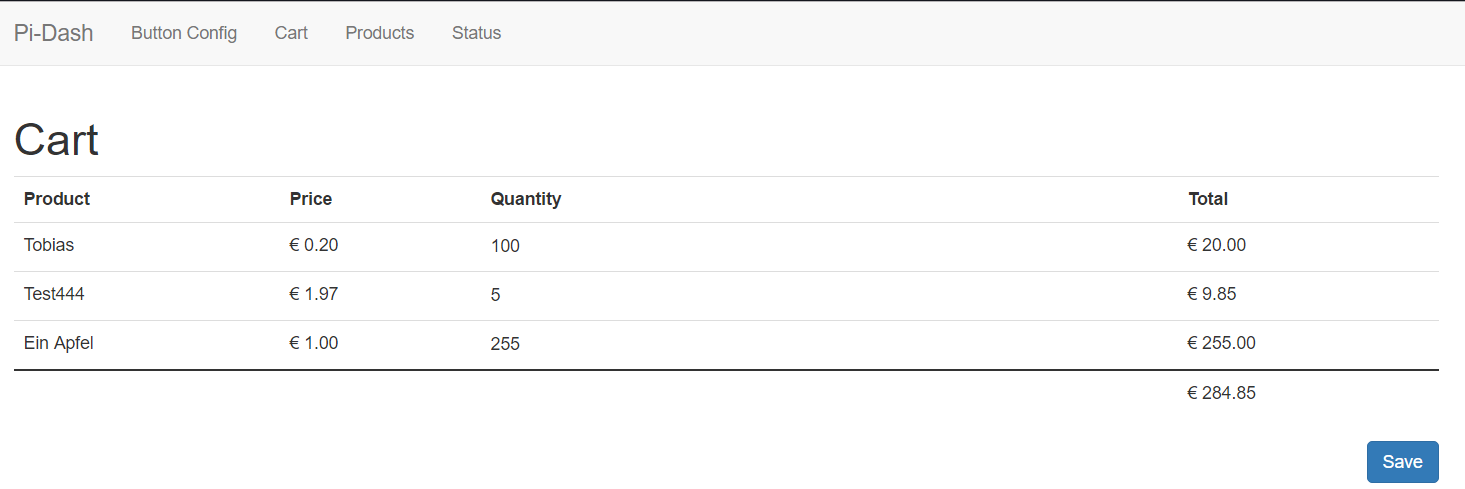
\includegraphics[scale=0.4]{Bilder/ui_cart.png}
	\caption[UI des Warenkorbs]{UI des Warenkorbs}
  \end{subfigure}\par\medskip
  \begin{subfigure}{\linewidth}	
	\centering
	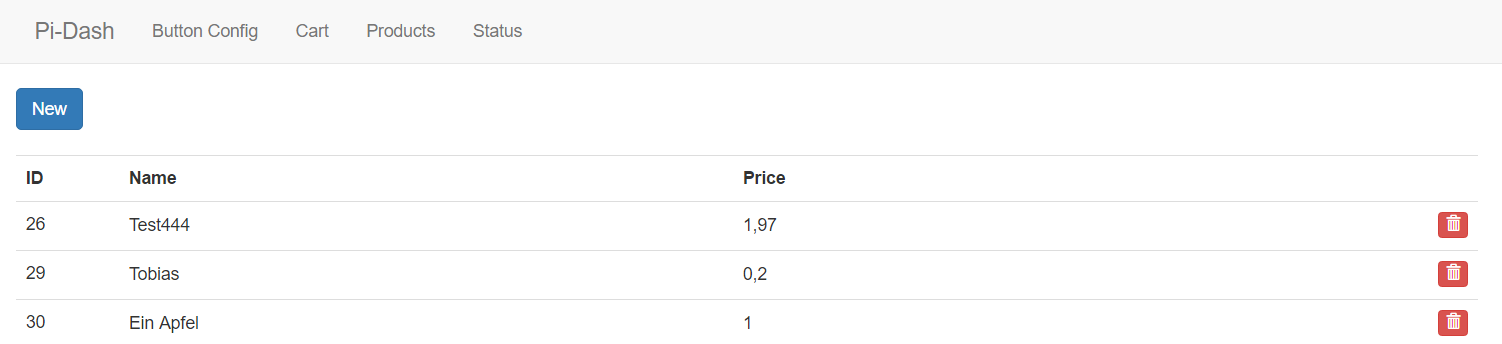
\includegraphics[scale=0.4]{Bilder/ui_products.png}
	\caption[UI der Produktübersicht]{UI der Produktübersicht}
  \end{subfigure}\par\medskip
  \begin{subfigure}{\linewidth}
	\centering
	
\includegraphics[scale=0.8]{Bilder/ui_status.png}
	\caption[UI der Statusseite]{UI der Statusseite}
  \end{subfigure}
  \caption{User Interface,\\ Quelle: Eigene Aufnahmen}
\end{figure}

